\subsection{STRUCTURE OF A METRIC SPACE}

Let X and \(X'\) be two metric spaces, d the metric on X, \(d'\) the metric on \(X'\) . In accordance with the general definitions (Set Theory, R, § 8, no. 5) a one-to-one mapping f of X onto \(X'\) is an isomorphism of the metric space structure of X onto that of \(X'\) if

\[
d (x, y) = d ^ {\prime} (f (x), f (y))\tag{1}
\]

for all \(x \in \mathbf{X}\) and all \(y \in \mathbf{X}\) .

Note that if \(f\) is a mapping of \(\mathbf{X}\) onto \(\mathbf{X}'\) which satisfies the identity (1), then \(f\) must be bijective and therefore an isomorphism of \(\mathbf{X}\) onto \(\mathbf{X}'\) ; such an isomorphism is also called an isometry (or an isometric mapping) of \(\mathbf{X}\) onto \(\mathbf{X}'\) .

\pandocbounded{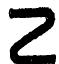
\includegraphics[keepaspectratio]{images/part001_40fd7be3.jpg}}

An isometry of X onto \(X'\) is of course an isomorphism of the uniformity (resp. topology) of X onto the uniformity (resp. topology) of \(X'\) ; the converses of these statements are false, as is shown by the existence of distinct equivalent metrics ( \(\S\) 1, no. 2).

Let X be a metric space, d the metric on X. For each a \textgreater{} 0 let \(V_{a}\) denote the subset of \(X \times X\) consisting of all pairs \((x, y)\) such that \(d(x, y) < a\) , and let \(W_{a}\) denote the subset of \(X \times X\) consisting of all pairs \((x, y)\) such that \(d(x, y) \leqslant a\) . As a runs through the set of all real numbers \textgreater{} 0 (or merely a sequence of numbers \textgreater{} 0 which tends to 0), the sets \(V_{a}\) (resp. \(W_{a}\) ) form a fundamental system of open (resp. closed) entourages of the uniformity of X, because of the continuity of d (§ 1, no. 3). We have \(\overline{V}_{a} \subset W_{a}\) , but these two sets are not necessarily the same.

By analogy with the case of the Euclidean distance on \(R^{n}\) , the set \(\mathrm{V}_{a}(x)\) {[}resp. \(\mathrm{W}_{a}(x)\) {]} is called the open (resp. closed) ball with centre x and radius a; it is an open (resp. closed) set in X. Again, the set of all \(y \in X\) such that \(d(x, y) = a\) is called the sphere with centre x and radius a; it is a closed set. From what has been said, the open (resp. closed) balls with centre x and radius a form a fundamental system of neighbourhoods of x as a runs through the set of all real numbers \textgreater0, or a sequence of numbers \textgreater0 which tends to o.

\pandocbounded{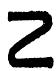
\includegraphics[keepaspectratio]{images/part001_d95d2d33.jpg}}

The reader should beware of assuming that balls and spheres in an arbitrary metric space enjoy the same properties as the Euclidean balls and spheres studied in Chapter VI, § 2. Thus the closure of an open ball need not be the closed ball of the same centre and radius; the frontier of a closed ball need not be the sphere of the same centre and radius; an open (or closed) ball need not be connected; and a sphere can be empty (cf.~Exercise 4).

Let A and B be any two non-empty subsets of a metric space X. The number

\[
d (\mathbf {A}, \mathbf {B}) = \inf _ {x \in \mathbf {A}, y \in \mathbf {B}} d (x, y)
\]

is called the distance between the sets A and B. In particular we denote by \(d(x, \mathbf{A})\) the distance between the set \(\{x\}\) and the set A; this is called the distance from the point x to the set A. Thus

\[
d (x, \mathrm{A}) = \inf _ {y \in \mathrm{A}} d (x, y)
\]

whence

\[
d (\mathbf {A}, \mathbf {B}) = \inf _ {x \in \mathbf {A}} d (x, \mathbf {B})
\]

(Chapter IV, § 5, no. 4, Proposition 9).

Remark. If \(d(x, \mathrm{A}) = a\) , it can happen that there is no point of A whose distance from \(x\) is equal to \(a\) . However, this situation can never arise if A is compact, for then Weierstrass's theorem (Chapter IV, §6, no. 1, Theorem 1) shows that there exists \(y \in \mathrm{A}\) such that \(d(x, \mathrm{A}) = d(x, y)\) .

PROPOSITION 2. The statements \(d(x, \mathbf{A}) = 0\) and \(x \in \overline{\mathbf{A}}\) are equivalent.

For \(d(x, \mathbf{A}) = 0\) expresses the fact that the ball \(\mathbf{V}_a(x)\) meets \(\mathbf{A}\) whatever the value of \(a > 0\) ; and this is equivalent to \(x \in \overline{\mathbf{A}}\) .

PROPOSITION 3. The function \(d(x, \mathbf{A})\) is uniformly continuous on \(\mathbf{X}\) .

Let \(x\) and \(y\) be any two points of \(\mathbf{X}\) ; then given any \(\varepsilon > 0\) there exists \(z \in \mathbf{A}\) such that \(d(y, z) \leqslant d(y, \mathbf{A}) + \varepsilon\) , and therefore

\[
d (x, z) \leqslant d (x, y) + d (y, z) \leqslant d (x, y) + d (y, A) + \varepsilon
\]

by the triangle inequality.

A fortiori \(d(x, \mathbf{A}) \leqslant d(x, y) + d(y, \mathbf{A}) + \varepsilon\) , and since \(\varepsilon\) is arbitrary it follows that \(d(x, \mathbf{A}) \leqslant d(x, y) + d(y, \mathbf{A})\) . Similarly we have

\[
d (y, \mathbf {A}) \leqslant d (x, y) + d (x, \mathbf {A}),
\]

so that

\[
\left| d (x, \mathbf {A}) - d (y, \mathbf {A}) \right| \leqslant d (x, y),\tag{2}
\]

whence the result follows.

Remark. We can have \(d(\mathbf{A}, \mathbf{B}) = 0\) for two subsets \(\mathbf{A}, \mathbf{B}\) of \(\mathbf{X}\) such that \(\overline{\mathbf{A}} \cap \overline{\mathbf{B}} = \emptyset\) , provided that neither subset consists of a single point. For example, on the real line \(\mathbf{R}\) , the set of integers \(> 0\) and the set of points of the sequence \((n + 1/2n)_{n \geqslant 1}\) are two disjoint closed sets whose distance apart is zero.

However, if A is compact and B is closed, the relation \(d(A, B) = 0\) implies \(A \cap B \neq \varnothing\) , for by virtue of the relation

\[
d (\mathbf {A}, \mathbf {B}) = \inf _ {x \in \mathbf {A}} d (x, \mathbf {B})
\]

it follows from Proposition 3 and Weierstrass's theorem that there exists \(x_0 \in \mathbf{A}\) such that \(d(x_0, \mathbf{B}) = d(\mathbf{A}, \mathbf{B}) = 0\) and hence (Proposition 2) \(x_0 \in \mathbf{B}\) .

The diameter of a non-empty subset A of X is the number (finite or equal to +∞)

\[
\delta (\mathbf {A}) = \sup _ {x \in \mathbf {A}, y \in \mathbf {A}} d (x, y).
\]

The notion of a ``W \(_{a}\) -small set'' (Chapter II, § 3, no. 1) is identical with that of a set of diameter \(\leqslant a\) . A non-empty set A consists of a single point if and only if \(\delta(\mathbf{A}) = 0\) .

A subset A of X is bounded (with respect to the metric d) if its diameter is finite; equivalently, if for each point \(x_{0} \in X\) , A is contained in a ball with centre \(x_{0}\) . Every subset of a bounded set is bounded, and the union of a finite family of bounded sets is a bounded set.

Note that a subset of X can be bounded with respect to a metric d but unbounded with respect to a metric equivalent to d (cf.~§ 1, no. 2).

